\newpage
\chapter{Flight Test}
\label{chap:flight_test}

\section{Flight Objectives and Planning}
%
Building and flying airships is not mentioned in many university text books. This suggests the U-SPACE project to follow a more empirical development approach were practical tests will confirm or discard the chosen design approaches. The objective of this first flight is to test suitability of the overall subsystem concepts. Specifically, we want to test:

\begin{itemize}
\item Motors capability to provide sufficient thrust to propel the blimp forward and steer it to the sides
\item Plausibility to provide all the required motor power from solar cells
\item Ground station communication link
\item In-flight functional test of EPS telemetry and telecommand 
\item Cargo bay mounting method
\item Ease and flexibility of complete system design when preparing and executing a flight, e.g. access to vital components, system diagnostics, system reset etc.
\item Logistics in preparation and execution of flight tests, e.g. access to equipment and spare parts etc.
\end{itemize}
%
%
\section{Flight Results}
\label{sec:flight_results}
%write for each subsystem
%
Figure \ref{fig:FlightTest1} shows two images taken from the first U-SPACE flight test on 14th of December 2012 at Esrange Space Center.
%
\begin{figure}
\begin{minipage}[t]{\linewidth}
\centering
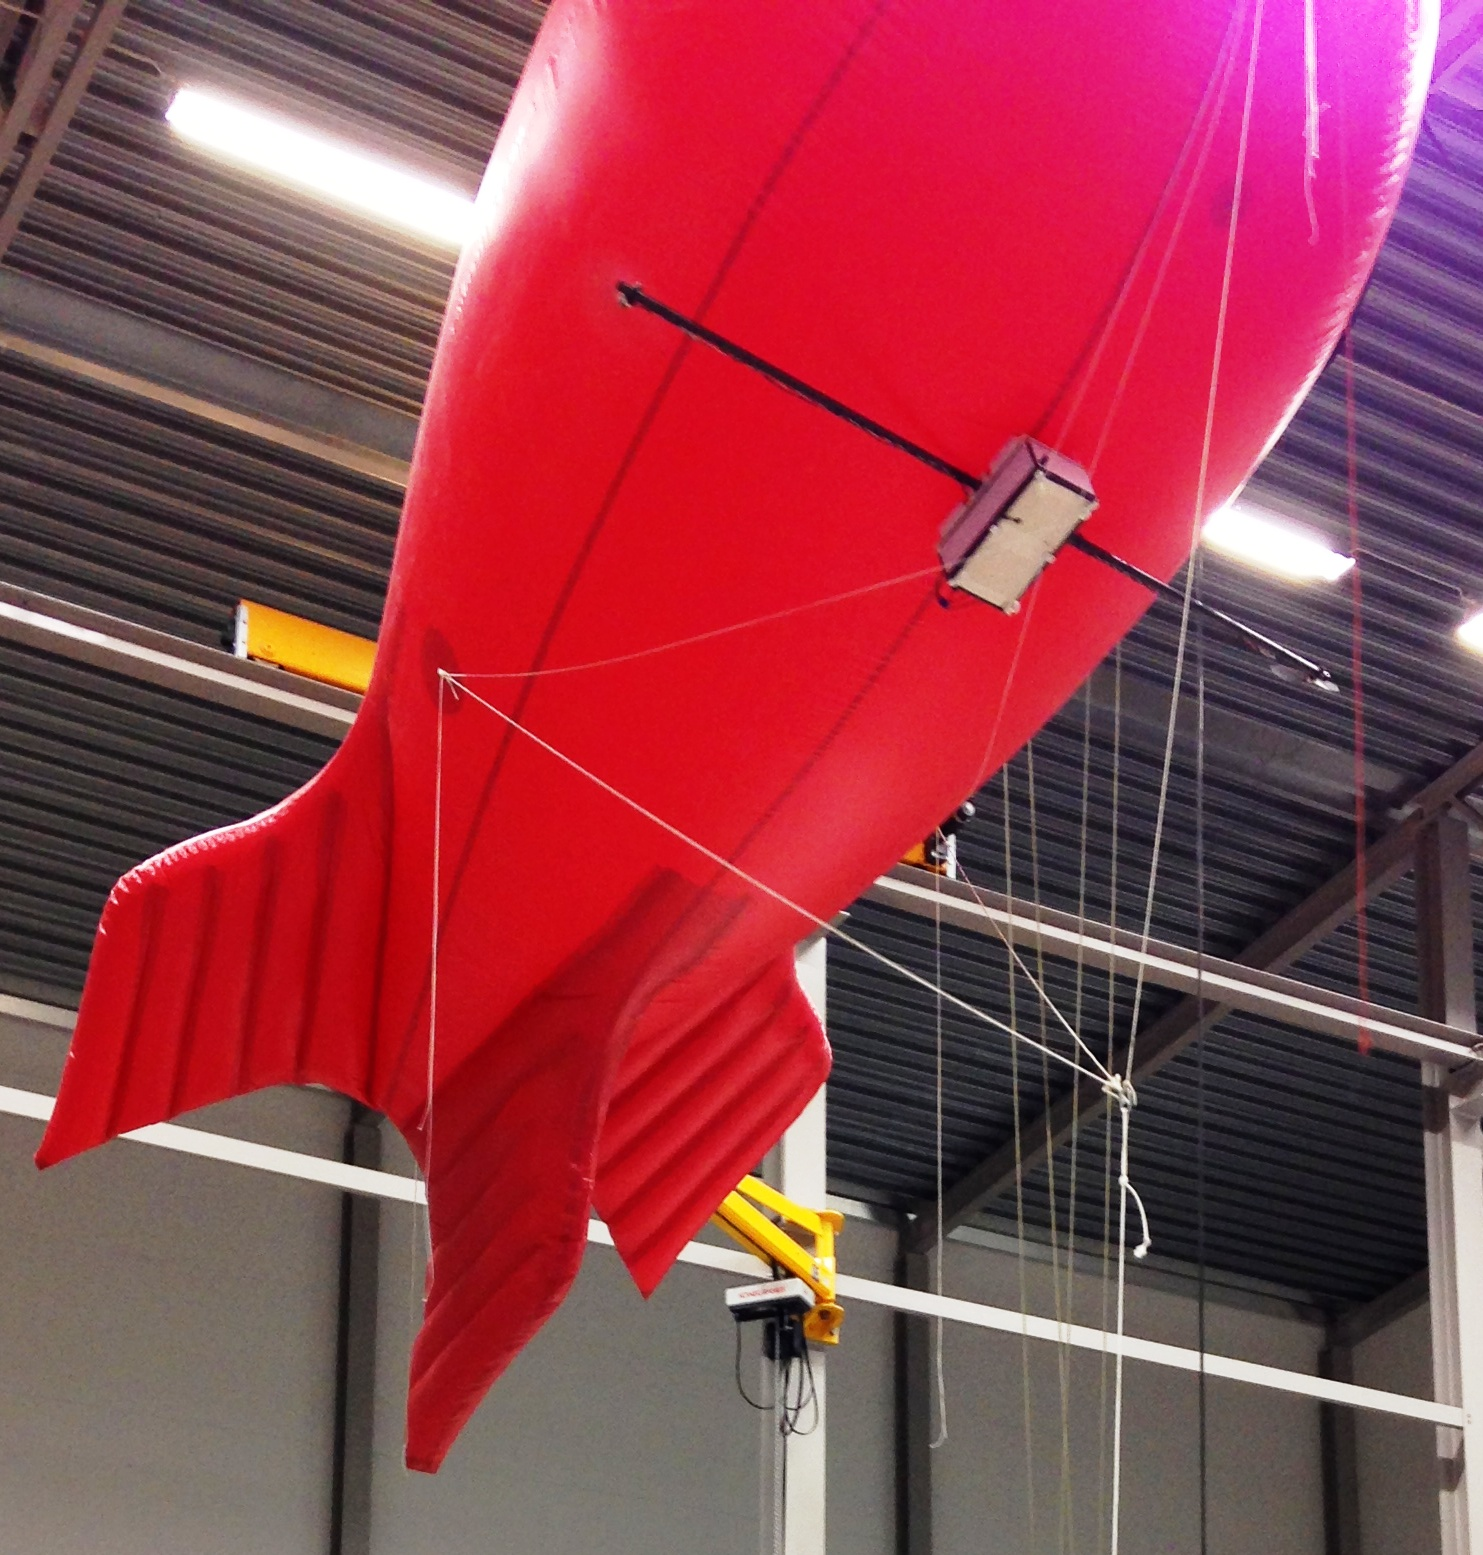
\includegraphics[width=0.7\textwidth]{figures/fig_FlightTest1_1}
\end{minipage}
\\[1mm]
\begin{minipage}[t]{\linewidth}
\centering
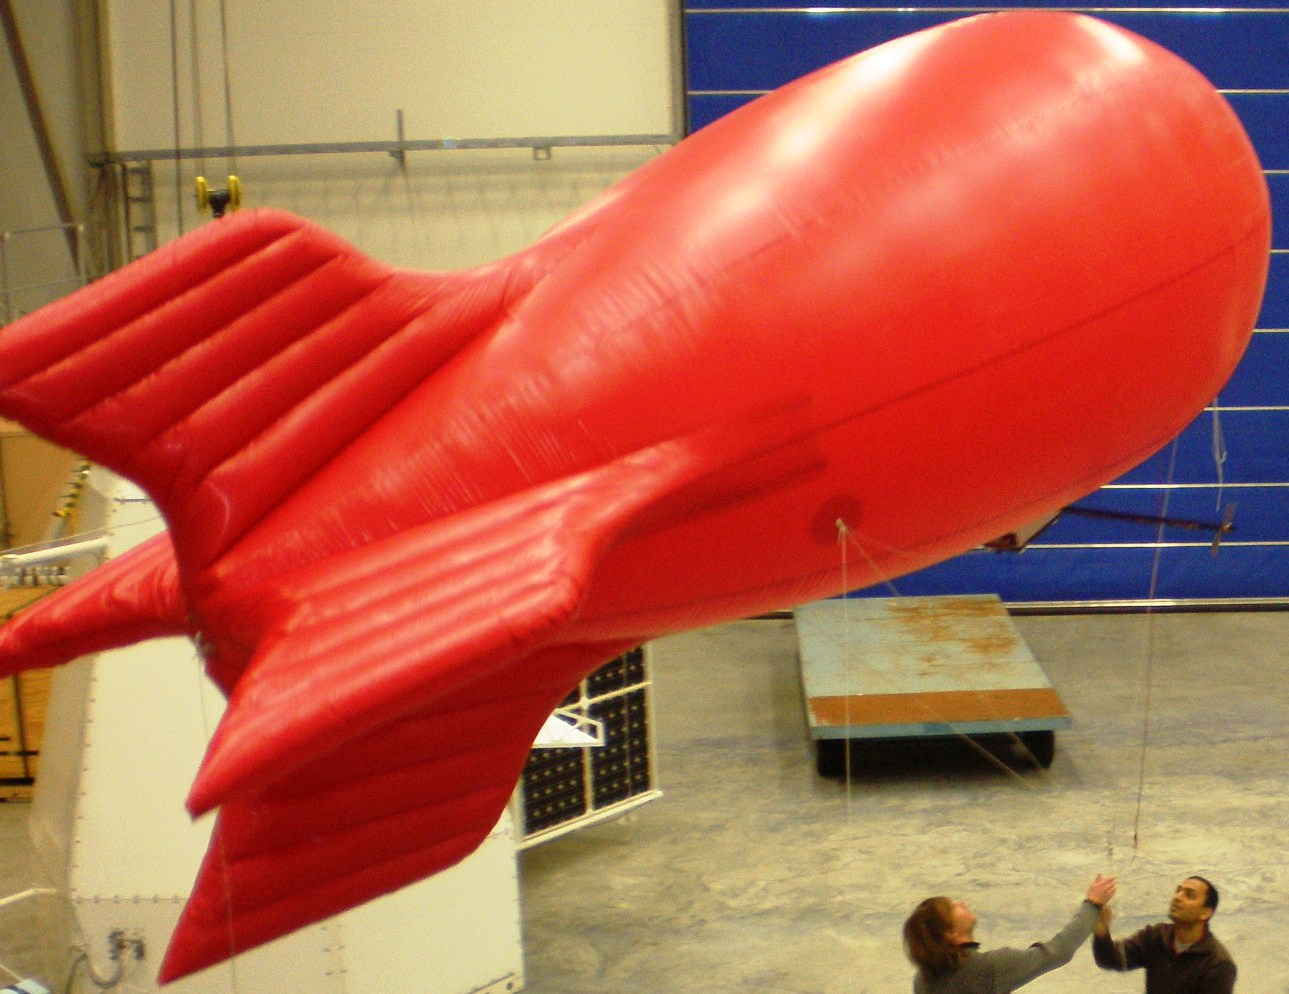
\includegraphics[width=0.7\textwidth]{figures/fig_FlightTest1_2}
\end{minipage}
\caption{First U-SPACE flight test at Esrange Space Center}
\label{fig:FlightTest1}
\end{figure}
%
%
The following sections describe the approaches and observations from this flight test.
%
\subsection{MSE}
The payload box structure behaved as expected during the mounting of the electronics payload, however an unexpected problem appeared while trying to attach it to the blimp.  An excessive traction load was applied to the frame by having the strings shown in the picture pulling too hard in opposite directions, which at some point became too much for the structure to withstand. Fortunately, the fracture occurred on one of the lower corners and that allowed an easy fix with adhesive tape which permitted us to continue the flight test as planned. 

We believe that this string attachment method is not well suited for the purpose of our project. It was obviously chosen for its combination of mounting versatility as it was already available from our basic materials and the fact that Esrange did not allow us to borrow the blimp to try different attaching systems at LTU. Therefore it was decided that without previous trials, this was the most effective way to attach the box and be able to ascertain that our project indeed flies. 
We used 3 attachment points; 2 of them located symmetrically on each side and one on the nose. They can be clearly seen on the pictures; they are the same points used to keep the balloon anchored to the ground.
Initially, the 4 clamps attached on each of the bottom corners of the box where used as rings to make the strings pass through. Each clamp on the rear side was attached to the anchoring point on the same side and the two on the front to the nose point. However as it has been mentioned, while tightening up the string system on the frame corners collapsed. Consequently, the attaching method was switched to that shown on the picture; only the front clamps where used to attach the entire box. With this method the strings that belong to the side attaching points press the box against the blimp surface, achieving a tight enough position for the box. 
Eventually the system fulfilled the objective of attaching the payload box and to proceed with the flying test. 


\subsection{MCC}
At full throttle on the motors, we were able to propel the blimp forward and steer it to the side. However, it was clear that the amount of thrust generated by the motors was insufficient to properly propel the blimp. During the flight test, the blimp was attached to a concrete block on the ground via. a thin rope. When flying forward, the rope would stretch at an angle w.r.t. zenith and thus pull back the blimp. This made it difficult to estimate exactly the maximum velocity possible to obtain with the applied motor thrust. In this test, no attempt was made to "balance" out the lift of the blimp to the total mass of the U-SPACE systems. 

\subsection{ITPU}
%
Shortly before the flight test the BB failed. The attempted provisory fix using a BB-xM turned out to unstable during the flight test (see also \ref{sec:changes_itpu}). While trying to fixate cable connections between the BB-xM and the expansion board cable broke and damaged the expansion board unable to repair on the test side. Therefore the test results presented here are taken from the pre-flight test which was done in the facilities of LTU Kiruna when the original BB was still operational.

\begin{figure}
\centering
\includegraphics[width=0.55\textheight]{figures/full-system-setup}
\caption{Full system setup}
\label{fig:full_system}
\end{figure}

\begin{figure}
\centering
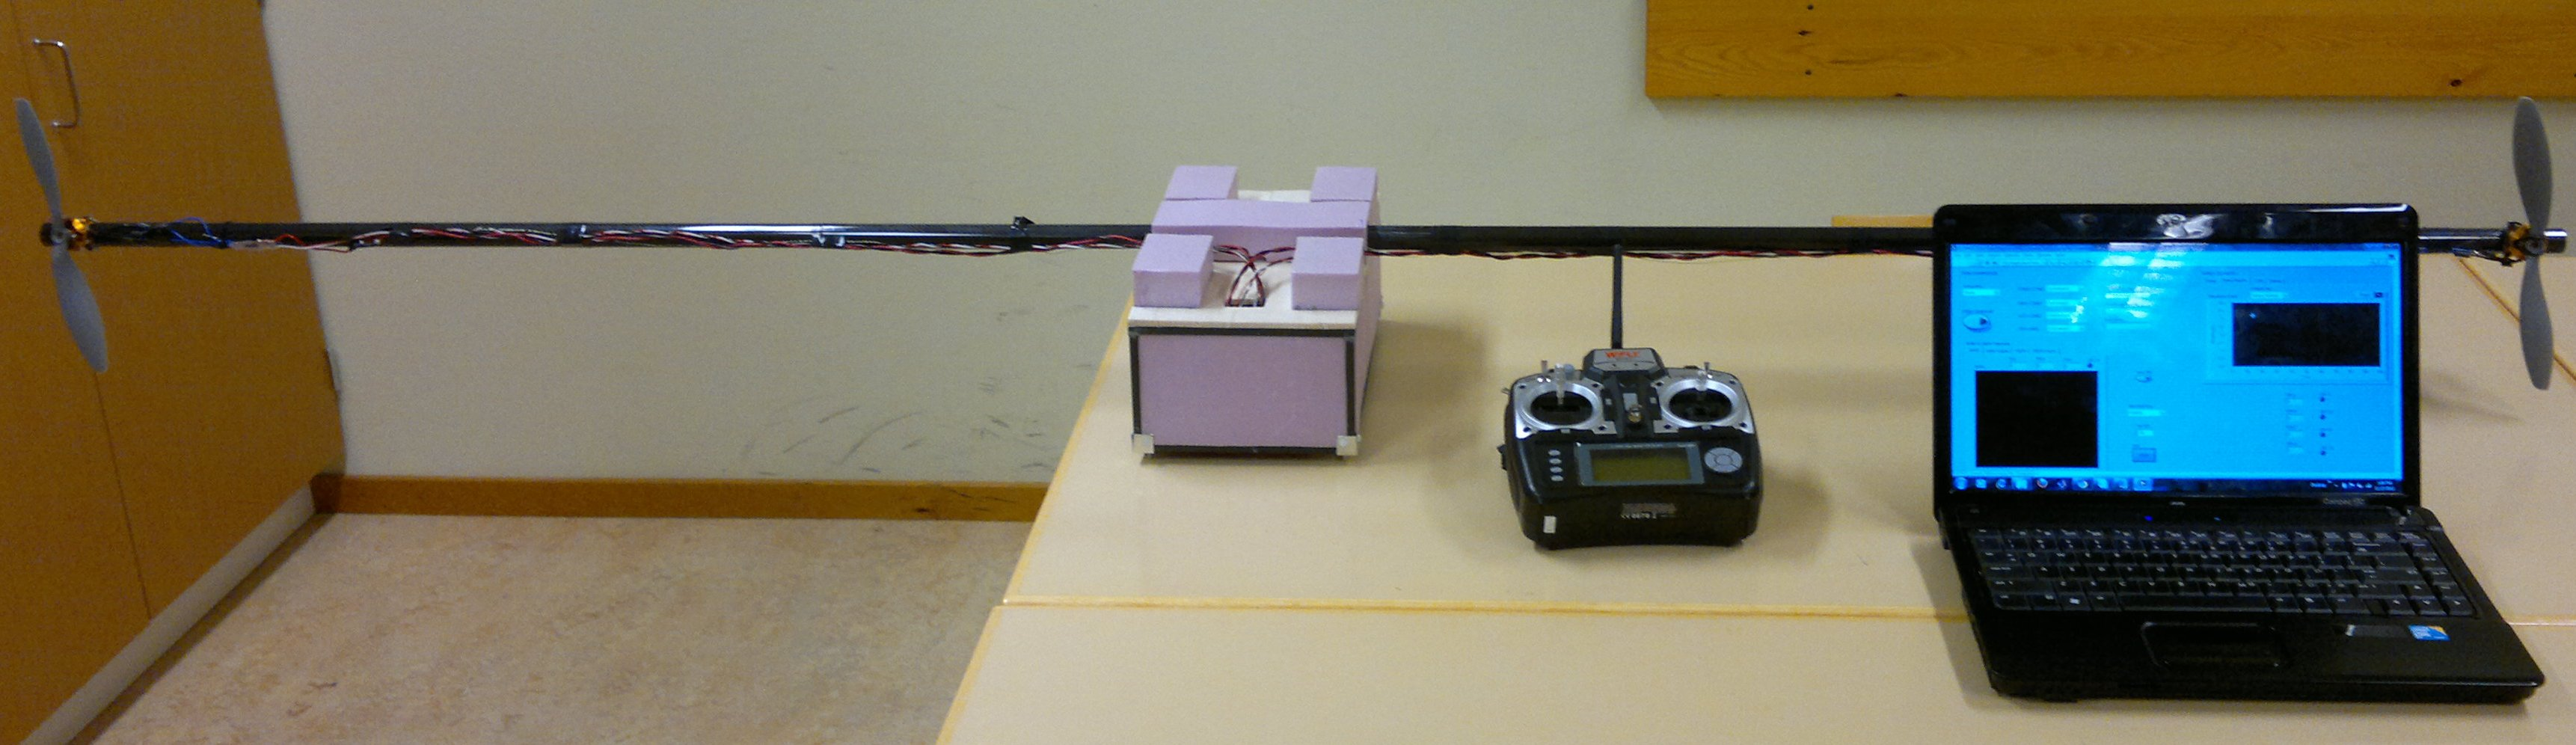
\includegraphics[width=\textwidth]{figures/fig_CargoBay}
\caption{Assembled Cargo Bay with electronics inside}
\label{fig:cargo_bay}
\end{figure}

An image of the full system setup including all electronic modules can be seen in figure \ref{fig:full_system}. This setup was then mounted into the payload box (see \ref{fig:cargo_bay}) for testing. As mentioned in section \ref{sec:changes_itpu}, operating both the ADCs of the telemetry subsystem and the sensors of the attitude determination subsystem on the same I2C-bus caused problems which needed manual reset of the I2C-bus in order to get it working again. Peculiar was that both system worked when only one of the two ADCs where connected to the I2C bus together with the attitude sensors, but failed when both ADCs were connected. As the attempts to enable a second I2C-bus on a different expansion header of the BB were unsuccessful, it was decided to test only with one ADC and in turn loose 8 of the 16 telemetry values of the internal voltages. 

With this decision implemented the testing went successful. The wireless connection to the ground station could be established. After calibration of the magnetometer, the attitude determination system was able to determine the attitude stably and produce the roll-, pitch- and yaw-angles for the telemetry system. When receiving the corresponding signal from the communication module the camera could be activated and shoot either single images or multiple images with a set period (fastest 1~s) and save them to the onboard SD-card.  

\subsection{EPS}
Due to the above discussed connector issues, no telemetry was obtained from the \ac{EPS}. However, power for motors and logic devices was available during the complete flight so it is concluded that the basic functionality of the \ac{EPS} worked fine. 

\subsection{Thermal Control}
The lack of telemetry meant that no temperatures were recorded. Hence, flight verification of the thermal design was not obtained.

\subsection{COM}

However, due to one bad solder connection in the voltage level conversion board, first flight testing was not carried out.

\section{Discussions and Future Recommendations}
%write for each subsystem
%
\subsection{MSE}
For future flights, the existing string attachment method will be discarded and replaced by a more easy-to-mount and effective way. In any case, in the event that this project is continued in the future, one of the first steps to take is the design and construction of a custom made envelope, which of course will be tailored to provide the right method of attaching their own subsystems, i.e. payload box, solar cells, propellers and so on. 

A custom made envelope would potentially acquire a higher lift-to-weight ratio, which would allow to incorporate heavier elements and more payload to the airship. This would  allow to build an aluminium based structure for the entire frame of the payload box, which not only would be much more resistant but also easier to build. 
A custom envelope will also allow to implement easier ways to attach the payload and the solar cells on top, without having to improvise a provisional rope attaching method taking several hours. 


\subsection{EPS}
Due to the connector issues discussed in section \ref{sec:flight_results}, no telemetry was available during flight, thus detailed information of power consumption were not obtained. However, at full thrust, the system has in laboratory shown to draw around 2 x 7.5 A. At a voltage of approximately 7.0 V this corresponds to 105 W power delivered to the motors. In \cite{CDR} the \ac{EPS} was designed to deliver minimum 40 W of continuous solar power. With these flight results, to allow continuous flight, future designs should increase the solar array power output by at least a factor 2.5-3.
 
The \ac{BCR} should be re-designed for higher voltage and current outputs. The chosen Li-ion battery can supply up to 66 A continuously or 88 A burst. The main limitation of the \ac{BCR} power output is due to current ratings on the power diode (20 A), power connectors (19 A) and wires (19 A or 11.5 A when using ECSS derating\cite{ECSS_derating}). PCB trace thickness may also become impractically thick at higher currents. 
To increase the output power rating, the best and first option is to use a higher battery voltage by connecting several batteries in series (or using a higher voltage battery pack with more cells in series). An advantage with higher voltage is that the power distribution efficiency is increased, since the diode voltage-drop losses and resistive losses ($I^2 \cdot R$) are relatively reduced when comparing to the total amount of handled power. 
The current rating can also be increased by using higher power connectors, thicker wire or several wires in parallel, higher power diodes or two diodes in parallel and using thicker PCB copper tracing, reducing trace length, increasing trace width and improving the thermal layout (adding lots of heat sinks and thermal connections). 

As has been suggested, more power will be needed for future designs. This means more solar cells. The solar cells suggested in \cite{CDR}, however very light-weight, are quite expensive and if 5-10 times more power is required, the solar cell cost will probably be the single most expensive of the complete project. Thus, significant efforts should go into finding cheaper solar cells or negotiating sponsor/donation options from the solar cell manufacturer. 

%Provisions for re-charging the battery while connected 
%
\subsection{MCC}
From the previous discussed flight results, it was shown that the amount of generated thrust was just barely able to move the blimp. According to \cite{website:ModelMotors}, the motors have a relatively poor efficiency of around 67\%, especially when operating at heavy loads (high currents + low \ac{RPM}). The TIF-250 blimp from Esrange has a volume of $15$ m$^3$ and thus an approximate lift of around 15 kg. Including the motor efficiency, the power-to-lift ratio is 4.7 W/kg. Calculating this ratio for the Zeppelins that flew during the 1930's\cite{website:graf_zeppelin} gives 15.4 W/kg for the LZ-129 Hindenburg and 19.2 W/kg for the LZ-127 Graf. Thus the U-SPACE design has a power-to-lift ratio about 3-4 times less than old commercial designs. This agrees well with the lack of motor power to properly propel the blimp. The Zeppelins were designed for a cruise speed around 125 km/h (35 m/s) which is of course faster than the U-SPACE requirement. For future designs, it is recommended to include more powerful motors designed for low speed, low \ac{RPM} and high torque like \cite{website:ModelMotors_AXI5360}. Larger motors will also require a larger solar array to provide the power.
In future flights, it is recommended to balance out the envelope lift using dead weights (sand, small rocks etc.) such to better estimate the flight performance of the motors.

